\documentclass[11pt,a4paper,oneside]{report}             % Single-side
%\documentclass[11pt,a4paper,twoside,openright]{report}  % Duplex

%\PassOptionsToPackage{chapternumber=Huordinal}{magyar.ldf}
\usepackage{t1enc}
\usepackage[utf8]{inputenc}
\usepackage{amsmath}
\usepackage{amssymb}
\usepackage{enumerate}
\usepackage[thmmarks]{ntheorem}
\usepackage{graphics}
\usepackage{epsfig}
\usepackage{listings}
\usepackage{color}
\usepackage{fancyhdr}
\usepackage{lastpage}
\usepackage{anysize}
\usepackage[magyar]{babel}
%\usepackage{indentfirst}
%\usepackage{natbib}
\usepackage{sectsty}
\usepackage{setspace}  % Ettol a tablazatok, abrak, labjegyzetek maradnak 1-es sorkozzel!
\usepackage[hang]{caption}
\usepackage{hyperref}
%\usepackage{bookmark}


%--------------------------------------------------------------------------------------
% Main variables
%--------------------------------------------------------------------------------------
\newcommand{\mitauthork}{Barta Pál}
\newcommand{\mitauthorkneptun}{M6E1QL}
\newcommand{\mitauthorkmail}{brazil.hu@gmail.com}
\newcommand{\mitauthor}{Kovács Dávid Balázs}
\newcommand{\mitauthorneptun}{JWMYNX}
\newcommand{\mitauthormail}{davidkovaccs@gmail.com}
\newcommand{\mitadvisor}{Dévai István}
\newcommand{\mitadvisortitle}{tanársegéd}
\newcommand{\mitadvisormail}{istvan.devai@aut.bme.hu}
\newcommand{\mittitle}{Tőzsdei rendszer}

%--------------------------------------------------------------------------------------
% Custom hyphenations
%--------------------------------------------------------------------------------------
\hyphenation{Silverlight}
\hyphenation{Windows}
\hyphenation{Microsoft}
\hyphenation{Intel}
\hyphenation{Linux}

%--------------------------------------------------------------------------------------
% Redefine original \chapter and \section commands
%--------------------------------------------------------------------------------------
\let\oldchap=\chapter
\renewcommand*{\chapter}{\secdef{\chapternostar}{\chapterstar}}
%\newcommand\chapterstar[1]{\oldchap*{#1}\markboth{~}{#1}\addcontentsline{toc}{chapter}{#1}}
\newcommand\chapterstar[1]{\phantomsection\addcontentsline{toc}{chapter}{#1}\oldchap*{#1}\markboth{~}{#1}}
%The first argument to \chapter is optional, hence the need for "[]"
%in the following definition. However, \secdef duplicates the mandatory
%argument if no optional argument was given. So we'll always have that
%argument and the default doesn't matter.
%\newcommand\chapternostar[2][]{\oldchap[#1]{#2}\markboth{\thechapter. #1}{\thechapter. #1}}
\newcommand\chapternostar[2][]{\phantomsection\oldchap[#1]{#2}\markboth{\thechapter. #1}{\thechapter. #1}}

\let\oldsect=\section
\renewcommand*{\section}{\secdef{\sectionnostar}{\sectionstar}}
%\newcommand\sectionstar[1]{\oldsect{#1}\markright{\thesection. #1}}
\newcommand\sectionstar[1]{\phantomsection\oldsect{#1}\markright{\thesection. #1}}
%\newcommand\sectionnostar[2][]{\oldsect[#1]{#2}\markright{\thesection. #1}}
\newcommand\sectionnostar[2][]{\phantomsection\oldsect[#1]{#2}\markright{\thesection. #1}}

\let\oldsubsect=\subsection
\renewcommand*{\subsection}{\secdef{\subsectionnostar}{\subsectionstar}}
\newcommand\subsectionstar[1]{\phantomsection\oldsubsect{#1}\markright{\thesection. #1}}
\newcommand\subsectionnostar[2][]{\phantomsection\oldsubsect[#1]{#2}\markright{\thesection. #1}}

\let\oldsubsubsect=\subsubsection
\renewcommand*{\subsubsection}{\secdef{\subsubsectionnostar}{\subsubsectionstar}}
\newcommand\subsubsectionstar[1]{\phantomsection\oldsubsubsect{#1}\markright{\thesection. #1}}
\newcommand\subsubsectionnostar[2][]{\phantomsection\oldsubsubsect[#1]{#2}\markright{\thesection. #1}}

%--------------------------------------------------------------------------------------
% Page layout setup
%--------------------------------------------------------------------------------------
% we need to redefine the pagestyle plain
% another possibility is to use the body of this command without \fancypagestyle
% and use \pagestyle{fancy} but in that case the special pages
% (like the ToC, the References, and the Chapter pages)remain in plane style
\fancypagestyle{plain}
{
	\fancyhead[R]{}
	\fancyhead[CO]{\bfseries\footnotesize\nouppercase{\rightmark}}
	\fancyhead[CE]{\bfseries\footnotesize\nouppercase{\leftmark}}
	\fancyhead[L]{}
	\fancyfoot[LE,RO]{}%\thepage}%{\thepage\pageref{LastPage}}
	\fancyfoot[C]{\thepage}
	\fancyfoot[LO,RE]{}
	\renewcommand{\headrulewidth}{0.4pt}
%	\renewcommand{\footrulewidth}{0.4pt}
}

\pagestyle{plain}
\setlength{\headheight}{15pt}
%\setlength{\parindent}{0pt} % áttekinthetőbb, angol nyelvű dokumentumokban jellemző
%\setlength{\parskip}{8pt plus 3pt minus 3pt} % áttekinthetőbb, angol nyelvű dokumentumokban jellemző
\setlength{\parindent}{12pt} % magyar nyelvű dokumentumokban jellemző
\setlength{\parskip}{0pt}    % magyar nyelvű dokumentumokban jellemző

\marginsize{35mm}{25mm}{15mm}{15mm} % anysize package
\setcounter{secnumdepth}{0}
%\setcitestyle{authoryear, round, comma, aysep={;}, yysep={,}, notesep={, }}
\sectionfont{\large\upshape\bfseries}

\setcounter{secnumdepth}{2}
\singlespacing
\frenchspacing

%--------------------------------------------------------------------------------------
%	Setup hyperref package
%--------------------------------------------------------------------------------------
\hypersetup{
    bookmarks=true,           % show bookmarks bar?
    bookmarksnumbered=true,   % set numbering
    unicode=true,             % non-Latin characters in Acrobat’s bookmarks
    pdftitle={\mittitle},     % title
    pdfauthor={\mitauthor, \mitauthork},   % author
    pdfsubject={házi feladat},% subject of the document
    pdfcreator={\mitauthor, \mitauthork},  % creator of the document
    pdfproducer={Producer},   % producer of the document
    pdfkeywords={családfa, family tree},   % list of keywords
    pdfnewwindow=true,        % links in new window
    colorlinks=true,          % false: boxed links; true: colored links
    linkcolor=black,          % color of internal links
    citecolor=black,          % color of links to bibliography
    filecolor=black,          % color of file links
    urlcolor=black            % color of external links
}
%--------------------------------------------------------------------------------------
%	Some new commands and declarations
%--------------------------------------------------------------------------------------
%\renewcommand{\captionfont}{\small\itshape}
%\renewcommand{\captionlabelfont}{\small\upshape\bfseries}
\newcommand{\code}[1]{{\upshape\ttfamily\scriptsize\indent #1}}
%\newcommand{\url}[1]{{\upshape\ttfamily\normalsize #1}}

% define references
\newcommand{\figref}[1]{\ref{fig:#1}.}
\renewcommand{\eqref}[1]{(\ref{eq:#1})}
\newcommand{\listref}[1]{\ref{listing:#1}.}
\newcommand{\sectref}[1]{\ref{sect:#1}.}
\newcommand{\tabref}[1]{\ref{tab:#1}.}

\DeclareMathOperator*{\argmax}{arg\,max}
%\DeclareMathOperator*[1]{\floor}{arg\,max}
\DeclareMathOperator{\sign}{sgn}
\DeclareMathOperator{\rot}{rot}
\definecolor{lightgray}{rgb}{0.95,0.95,0.95}

\author{\mitauthor, \mitauthork}
\title{\mittitle}
\includeonly{
	preliminaries,%
	%introduction,%
	chapter1,%
	%chapter2,%
	%chapter3,%
	%assessment,%
}
%--------------------------------------------------------------------------------------
%	Setup captions
%--------------------------------------------------------------------------------------
\captionsetup[figure]{
%labelsep=none,
%font={footnotesize,it},
%justification=justified,
width=.75\textwidth,
aboveskip=10pt}

\renewcommand{\captionlabelfont}{\small\bf}
\renewcommand{\captionfont}{\footnotesize\it}

%--------------------------------------------------------------------------------------
% Table of contents and the main text
%--------------------------------------------------------------------------------------
\begin{document}

\singlespacing
%--------------------------------------------------------------------------------------
%	The title page
%--------------------------------------------------------------------------------------
\begin{titlepage}
\begin{center}

\includegraphics[width=100mm,keepaspectratio]{figures/BMElogo.png}\\
\textsc{Budapesti Műszaki és Gazdaságtudományi Egyetem}\\
\textsc{Automatizálási és Alkalmazott Informatikai Tanszék}\\[5cm]

\vspace{0.4cm}
{\huge \bfseries \mittitle}\\[0.8cm]
\vspace{0.5cm}
\textsc{\Large Szoftverarchitektúrák (VIAUM105)\\ Házi feladat}\\[4cm]

\begin{tabular}{cc}
 \makebox[7cm]{\emph{Készítették}} & \makebox[7cm]{\emph{Konzulens}} \\
 \makebox[7cm]{\mitauthor} & \makebox[7cm]{\mitadvisor} \\
 \makebox[7cm]{\mitauthorneptun} & \makebox[7cm]{\begin{small}\mitadvisortitle\end{small}} \\
 \makebox[7cm]{\url{\mitauthormail}} & \makebox[7cm]{\url{\mitadvisormail}} \\
 & \\
 \makebox[7cm]{\mitauthork} & \\
 \makebox[7cm]{\mitauthorkneptun} & \\
 \makebox[7cm]{\url{\mitauthorkmail}} & \\
\end{tabular}

\vfill
{\large \today}
\end{center}
\end{titlepage}

%--------------------------------------------------------------------------------------
% Set up listings
%--------------------------------------------------------------------------------------
\lstset{
	basicstyle=\scriptsize\ttfamily, % print whole listing small
	keywordstyle=\color{black}\bfseries\underbar, % underlined bold black keywords
	identifierstyle=, 					% nothing happens
	commentstyle=\color{white}, % white comments
	stringstyle=\scriptsize\sffamily, 			% typewriter type for strings
	showstringspaces=false,     % no special string spaces
	aboveskip=3pt,
	belowskip=3pt,
	columns=fixed,
	backgroundcolor=\color{lightgray},
} 		
\def\lstlistingname{lista}

%\newpage\thispagestyle{empty} % an empty page

%--------------------------------------------------------------------------------------
% Nyilatkozat
%--------------------------------------------------------------------------------------
\begin{center}
\pagenumbering{Roman}
%\clearpage
\phantomsection
\addcontentsline{toc}{chapter}{Hallgatói nyilatkozat}
\large
\textbf{HALLGATÓI NYILATKOZAT}\\
\end{center}

Alulírott \emph{\mitauthor} és \emph{\mitauthork}, a  Budapesti Műszaki és Gazdaságtudományi Egyetem hallgatói kijelentjük, hogy ezt a házi feladatot meg nem engedett segítség nélkül, saját magunk készítettük el.

\begin{flushleft}
\vspace*{1cm}
Budapest, \today
\end{flushleft}

\begin{flushright}
 \vspace*{1cm}
 \begin{tabular}{cc}
 \makebox[7cm]{\rule{6cm}{.4pt}} & \makebox[7cm]{\rule{6cm}{.4pt}} \\
 \makebox[7cm]{\emph{\mitauthor}} & \makebox[7cm]{\emph{\mitauthork}} \\
 \makebox[7cm]{hallgató} & \makebox[7cm]{hallgató} \\
 \end{tabular}
\end{flushright}
%\thispagestyle{empty}

\vfill
%\clearpage
%\thispagestyle{empty} % an empty page


\tableofcontents\vfill\markboth{Tartalomjegyzék}{~}


\onehalfspacing

\clearpage

\setcounter{page}{1}
\pagenumbering{arabic}
%%----------------------------------------------------------------------------
\chapter*{Bevezető}
%----------------------------------------------------------------------------

Családfákon\footnote{\url{http://hu.wikipedia.org/wiki/Csal\%C3\%A1dfa}} az ősök és utódok közötti kapcsolatokat jeleníthetjük meg, ezzel a családfa a származástan (genealógia) tudományában használt egyik fontos és szemléletes eszköz. Segítségével könnyedén eligazodhatunk a családi leszármazások szövevényén, netán megőrizhetjük az utókornak őseink emlékét. A régebbi időkben a családfákat ábrázoló festmények, falikárpitok komoly művészi értéket képviseltek (lásd \figref{bitto_csaladfa} ábra), mára azonban leginkább a családfa információtartalmát tartjuk szem előtt.

\begin{figure}[!ht]
\centering
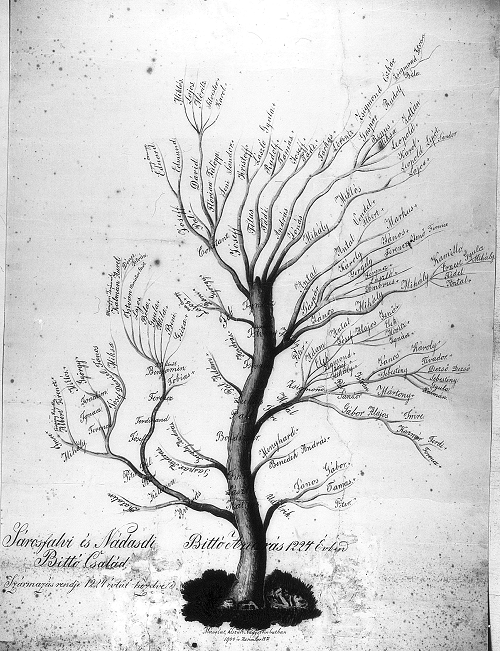
\includegraphics[width=70mm, keepaspectratio]{figures/bitto_csaladfa.png}
\caption{A Bittó család régi típusú családfája.}
\label{fig:bitto_csaladfa}
\end{figure}

Alapvetően a családfák két típusát különböztetjük meg.

\begin{itemize}
 \item Egy meghatározott személy őseit bemutató családfa; ez általában, mint egy fa koronája, felfelé növekszik.
 \item Egy személy (vagy pár) leszármazottait bemutató családfa; formája pont ellentétes az előzőéhez képest, akárcsak a fa gyökérzete, ,,lefelé'' növekszik.
\end{itemize}

Természetesen a fenti két típus kombinációja is elképzelhető, azonban ez ,,offline'' megoldásban nagyon gyorsan kezelhetetlenné és átláthatatlanná válhat. Szoftveres segítséggel azonban akár a bővebb családunk több generációt felölelő teljes családfáját is könnyedén megszerkeszthetjük és karban tarthatjuk. Sőt, akár olyan (pl. multimédiás) anyagokat tárolhatunk a családfában szereplő személyek mellett szinkronban, amelyek további információkkal és emlékekkel tudják teljessé tenni az ábrázolt család (akár a saját családunk) történetét.

%----------------------------------------------------------------------------
\chapter{Követelményspecifikáció}\label{sect:kovspec}
%----------------------------------------------------------------------------
A feladatunk egy tőzsdei kereskedési rendszer megvalósítása egy fejlett alkalmazás keretrendszer és többrétegű architektúra segítségével. A fejezet elején \sectref{defs} definiáljuk az alkalmazás fejlesztése közben előkerülő fogalmakat, majd bemutatjuk a különböző felhasználó típusokat akik használhatják a rendszert.
A \sectref{use_case} fejezetben bemutatjuk a legfontosabb felhasználói eseteket, majd a \sectref{all_use_case} fejezetben felsoroljuk az összes funkciót amit a rendszer támogatni fog. A \sectref{ui_design} részben felvázoljuk hogyan fognak kinézni a legfontosabb funkciók a képernyőn, illetve milyen lesz a képernyő elrendezése.
A fejezet végén röviden kitérünk az alkalmazás használata során felmerülő biztonsági problémákra \sectref{security}, majd bemutatjuk a tervezett architektúrát \sectref{designed_architecture}.

%,,,,,,,,,,,,,,,,,,,,,,,,,,,,,,,,,,,,,,,,,,,,,,,,,,,,,,,,,,,,,,,,,,,,,,,,,,,,
\section{Definíciók}\label{sect:defs}
%,,,,,,,,,,,,,,,,,,,,,,,,,,,,,,,,,,,,,,,,,,,,,,,,,,,,,,,,,,,,,,,,,,,,,,,,,,,,

\subsection{Felhasználó}
A rendszert felhasználók használják akiknek authentikálniuk kell magukat a rendszerbe való belépéshez. Minden felhasználóról tároljuk a nevét, a jogosultági körét és a jelszavát. Három féle felhasználót különböztetünk meg: \emph{ügyfél}, \emph{bróker}, \emph{adminisztrátor}.
\newline \underline{Adatok}: email cím, előnév, utónév, jelszó, szerepkör
\newline \underline{Megkötések}: kötelező a név, jelszó, email cím, szerepkör megadása

\subsection{Ügyfél}
Az ügyfél egy felhasználó. Miután beléptek a rendszerbe látják az árfolyamok aktuális alakulását és \emph{megbízásokat} köthetnek (vétel-eladás) bizonyos \emph{tőzsdei instrumentumra}. Lehetőségük van több \emph{számlát} fenntartani és mindegyikről külön \emph{megbízásokat} kötni, de legalább egy \emph{számlájuknak} kötelező lenni. Listázhatja éppen futó \emph{megbízásait} vagy nyomon követheti aktuális \emph{ügyleteit}.
\newline \underline{Megkötések}: legalább egy számlája van
\newline \underline{Adatok}: számlák, megbízások, ügyletek

\subsection{Tőzsdei instrumentum}
A tőzsdén jegyzett és kereskedhető eszközök, amikkel az ügyfelek kereskedhetnek a rendszer segítségével, eladási vagy vételi \emph{megbízásokat} köthetnek rájuk. Az áruk folyamatosan valós időben megjelenik az ügyfél előtt.
\newline \underline{Adatok}: aktuális ár

\subsection{Számla}
Minden ügyfélnek van legalább egy számlája, de akár több is. A számlának van egy \emph{egyenlege} ami az aktuálisian felhasználható pénz mennyisége. Minden számlához tartoznhatnak \emph{megbízások}, \emph{ügyletek}. Egy vételi megbízás indításakor a számláról lekerül a fedezet, majd ha az ügylet záros határidőn belül nem jön létre, a pénz visszakerül, egyébként végleg lekerül. Ha egy eladás ügylet létrejön az áru ára rákerül a az adott számlára (ahonnan az véve lett).
\newline \underline{Megkötések}: nem létezhet ügyfél nélkül
\newline \underline{Adatok}: egyenleg, megbízások, ügyletek

\subsection{Egyenleg}
A számlán aktuálisan található \emph{pénz összege}. Maximum ekkora értékű megbízás indítható az adott számláról.
\newline \underline{Adatok}: pénz összeg
\newline \underline{Megkotesek}: minden számlához tartozik

\subsection{Megbízás}
Egy megbízás lehet \emph{eladás} vagy \emph{vétel} egy adott tőzsdei instrumentumra, amelyet az ügyfél kezdeményez adott áron, adott mennyiségre. Ha két ellentétes tipusú és ugyanolyan áru megbízás találkozik akkor létrejön egy \emph{ügylet}. A mennyiségek osztódhatnak több ügyletre.
\newline \underline{Megkötések}: számlához tartozik (így ügyfélhez is)
\newline \underline{Adatok}: számla, instrumentum neve, mennyiség, ár, típus(vétel/eladás), kezdeményezés dátuma

\subsection{Ügylet}
Ha két ellentétes tipusú \emph{megbízás} történik egy idő intervallumban létrejön egy ügylet és a tőzsdei instrumentum gazdát cserélnek. A vevő számlájáról végleg lekerül a pénz, míg az eladóéra rákerül.
\newline \underline{Adatok}: két megbízás, mennyiség, dátum amikor létrejött
\newline \underline{Megkötések}: két ellentétes tipusú ügylet kell hozzá

\subsection{Bróker}
A bróker egy felhasználó. Megnézheti egy adott \emph{ügyfél} \emph{számláit} élő vagy inaktív \emph{megbízásait}, \emph{ügyleteit}.

\subsection{Adminisztrátor}
Az ügyfelek, brókerek \emph{regisztrációját} végzi a rendszerbe. Akár \emph{deaktiválhatja} is felhasználókat, ő a rendszer ura.


%,,,,,,,,,,,,,,,,,,,,,,,,,,,,,,,,,,,,,,,,,,,,,,,,,,,,,,,,,,,,,,,,,,,,,,,,,,,,
\section{Felhasználói szerepkörök}\label{sect:roles}
%,,,,,,,,,,,,,,,,,,,,,,,,,,,,,,,,,,,,,,,,,,,,,,,,,,,,,,,,,,,,,,,,,,,,,,,,,,,,

Mint fentebb már említettük három különböző felhasználói szerepkört különböztetünk meg a rendszerben.

\subsection{Ügyfél}
Miután belép látja az aktuális árfolyamokat és eladási vagy vételi megbízást indíthat akár azonnal. Listázni tudja a megbízásait, visszavonni, módosítani, látja a régebbi ügyleteit. Szintén listázni tudja a számláit, látja az aktuális egyenlegét, új számlákat tud létrehozni, tud utalni pénzt a számlájára.

\subsection{Bróker}
Látja az összes ügyfél adatait, megbízásait, ügyleteit, számláit.

\subsection{Adminisztrátor}
Rendelkezik ugyanazokkal a szerepekkel, mint egy bróker, de képes regisztrálni brókert, ügyfelet vagy akár törölheti is őket a rendserből.

%,,,,,,,,,,,,,,,,,,,,,,,,,,,,,,,,,,,,,,,,,,,,,,,,,,,,,,,,,,,,,,,,,,,,,,,,,,,,
\section{Leggyakoribb felhasználói esetek}\label{sect:use_case}

\subsection{Regisztráció kérelme}
A felhasználó egy felületen a szükséges adatok bevitelével regisztrációt kérvényez ami az adminisztrátorhoz kerül felülvizsgálatra. Az adminisztrátor engedélyezheti, elvetheti a kérelmet.
\newline \underline{Szerepkör}: Ügyfél, Adminisztrátor, Bróker

\subsection{Megbízás adása}
A felhasználó kitölt egy megbízási formulát, melyhez megadja a szükséges adatokat(instrumentum, mennyiség, eladás/vétel, ár), majd ezt beregisztrálja a rendszerbe.
\newline \underline{Szerepkör}: Ügyfél

\subsection{Megbízás visszavonása}
A felhasználó eltávolít egy megbízást.
\newline \underline{Szerepkör}: Ügyfél

\subsection{Ügyfél megbízásainak listázása}
A felhasználó kilistázza egy lapozható listában az összes aktív/inaktív megbízását.
\newline \underline{Szerepkör}: Bróker, Ügyfél (csak a sajátját)

\subsection{Ügyfél ügyleteinek historikus listázása}
A felhasználó kilistázza egy lapozható listában az összes ügyletet, ami az ügyfél megbízásai által jött létre. Az ügyleteket szűrhetjük aszerint, hogy eladók vagy vásárló az ügyfél.
\newline \underline{Szerepkör}: Bróker, Ügyfél (csak a sajátját)

%,,,,,,,,,,,,,,,,,,,,,,,,,,,,,,,,,,,,,,,,,,,,,,,,,,,,,,,,,,,,,,,,,,,,,,,,,,,,
\section{Funkciók}\label{sect:all_use_case}
%,,,,,,,,,,,,,,,,,,,,,,,,,,,,,,,,,,,,,,,,,,,,,,,,,,,,,,,,,,,,,,,,,,,,,,,,,,,,

\subsection{Regisztráció kérelme}
A felhasználó egy felületen a szükséges adatok bevitelével regisztrációt kérvényez
\newline \underline{Szerepkör}: Ügyfél, Adminisztrátor, Bróker

\subsection{Felhasználó regisztrációja}
A felhasználó a beérkezett regisztrációs kérelmet feldolgozza és létrehoz egy új felhasználót, a role alapvetően ügyfél típusú lesz
\newline \underline{Szerepkör}: Adminisztrátor

\subsection{Felhasználó kinevezése}
Az felhasználó kinevezhet egy ügyfelet brókernek vagy adminisztrátornak
\newline \underline{Szerepkör}: Adminisztrátor

\subsection{Felhasználó deaktiválása}
A felhasználó eltávolíthat egy felhasználót és annak összes bejegyzését a rendszerből
\newline \underline{Szerepkör}: Adminisztrátor

\subsection{Ügyfél számla létrehozása}
Az felhasználó az adott ügyfél számára létrehoz egy számlát
\newline \underline{Szerepkör}: Adminisztrátor

\subsection{Ügyfél számla módosítása}
A felhasználó módosítja az ügyfélhez tartozó számlát
\newline \underline{Szerepkör}: Adminisztrátor

\subsection{Ügyfél számla törlése}
A felhasználó eltávolít egy ügyfél számlát
\newline \underline{Szerepkör}: Adminisztrátor

\subsection{Megbízás adása}
 A felhasználó kitölt egy megbízási formulát, melyhez megadja a szükséges adatokat, majd ezt beregisztrálja a rendszerbe.
\newline \underline{Szerepkör}: Ügyfél

\subsection{Megbízás módosítása}
A felhasználó módosítja az egyik megbízást.
\newline \underline{Szerepkör}: Ügyfél

\subsection{Megbízás visszavonása}
A felhasználó eltávolít egy megbízást.
\newline \underline{Szerepkör}: Ügyfél

\subsection{Ügyfél ügyleteinek historikus listázása}
A felhasználó kilistázza egy lapozható listában az összes ügyletet, ami az ügyfél megbízásai által jött létre. Az ügyleteket szűrhetjük aszerint, hogy eladók vagy vásárló az ügyfél.
\newline \underline{Szerepkör}: Bróker, Ügyfél (csak a sajátját)

\subsection{Ügyfél számláinak megtekintése}
A felhasználó lekéri egy adott ügyfél összes számlájának listáját.
\newline \underline{Szerepkör}: Bróker, Ügyfél (csak a sajátját)

\subsection{Ügyfél számlaegyenlegének megtekintése}
A bróker lekéri egy adott ügyfél adott számlájának egyenlegét.
\newline \underline{Szerepkör}: Bróker, Ügyfél (csak a sajátját)

\subsection{Ügyfél élő megbízásainak megtekintése}
A bróker lekéri egy adott ügyfél élő megbízásait.
\newline \underline{Szerepkör}: Bróker, Ügyfél (csak a sajátját)

\subsection{Ügyfél inaktív megbízásainak megtekintése}
A bróker lekéri egy adott ügyfél inaktív megbízásait.
\newline \underline{Szerepkör}: Bróker, Ügyfél (csak a sajátját)

\newpage
%,,,,,,,,,,,,,,,,,,,,,,,,,,,,,,,,,,,,,,,,,,,,,,,,,,,,,,,,,,,,,,,,,,,,,,,,,,,,
\section{Felhasználói interfész tervek}\label{sect:ui_design}
%,,,,,,,,,,,,,,,,,,,,,,,,,,,,,,,,,,,,,,,,,,,,,,,,,,,,,,,,,,,,,,,,,,,,,,,,,,,,


\subsection{Regisztráció}

\begin{figure}[!ht]
\centering
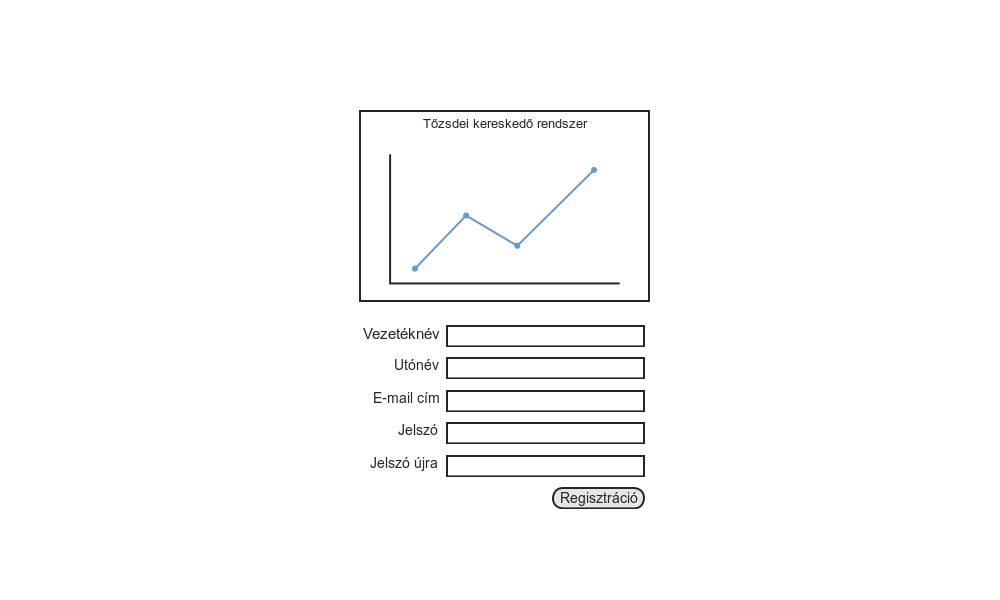
\includegraphics[width=150mm, keepaspectratio]{figures/user_1/register.png}
\caption{Regisztráció}
\label{fig:haromreteg}
\end{figure}

\subsection{Bejelentkezés}

\begin{figure}[!ht]
\centering
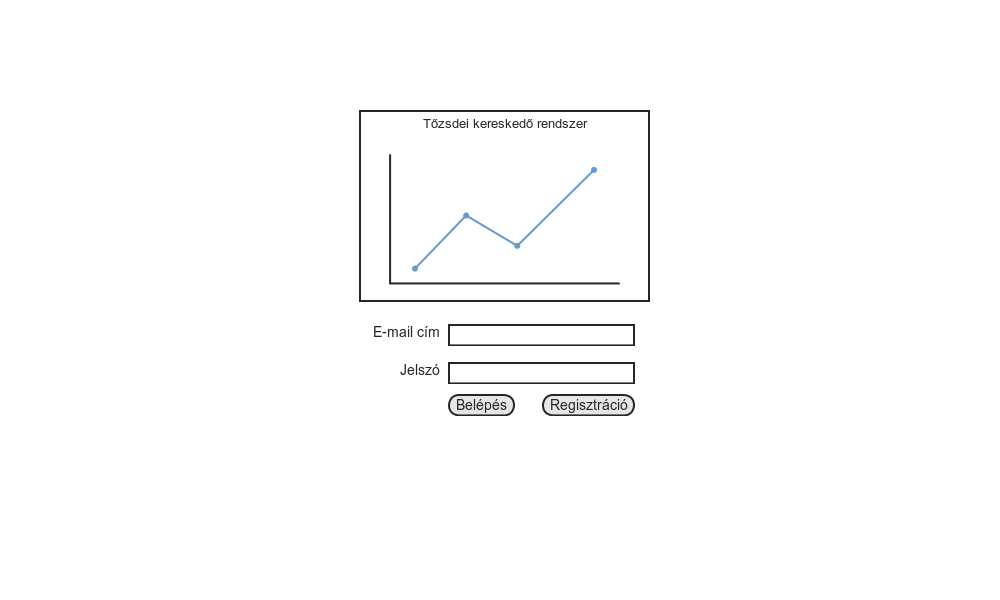
\includegraphics[width=150mm, keepaspectratio]{figures/user_1/login.png}
\caption{Bejelentkezés}
\label{fig:haromreteg}
\end{figure}

\subsection{Felhasználók menedzselése}

Az adminisztrátor ezen az oldalon tudja karbantartani a felhasználókat.

\begin{figure}[!ht]
\centering
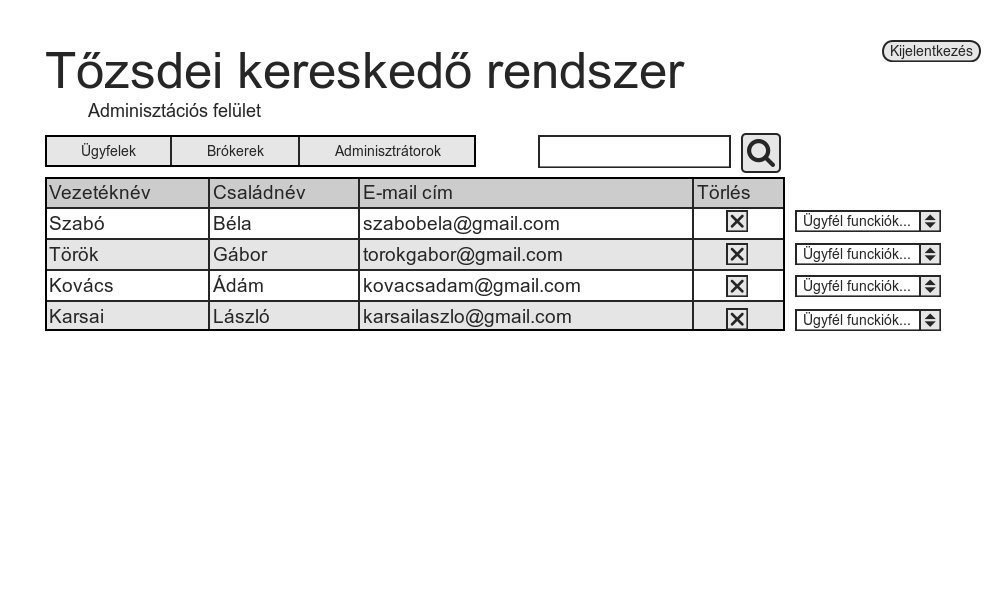
\includegraphics[width=150mm, keepaspectratio]{figures/user_1/admin_users.png}
\caption{Felhasználók menedzselése}
\label{fig:haromreteg}
\end{figure}

\subsection{Ügyfél kezdőlapja}

\begin{figure}[!ht]
\centering
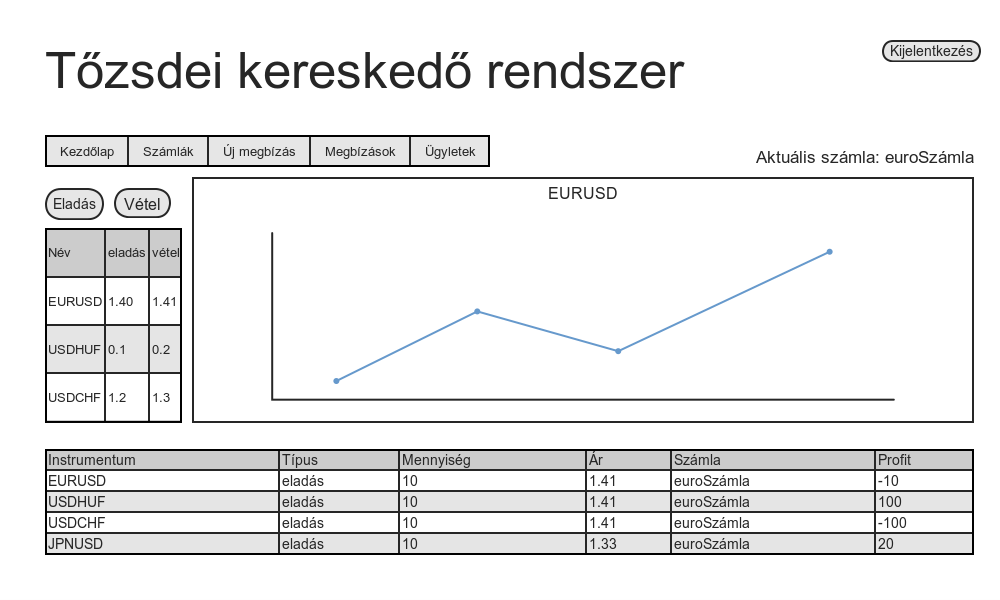
\includegraphics[width=150mm, keepaspectratio]{figures/user_1/Home.png}
\caption{Ügyfél kezdőlapja}
\label{fig:haromreteg}
\end{figure}

\subsection{Ügyfél számlái}

\begin{figure}[!ht]
\centering
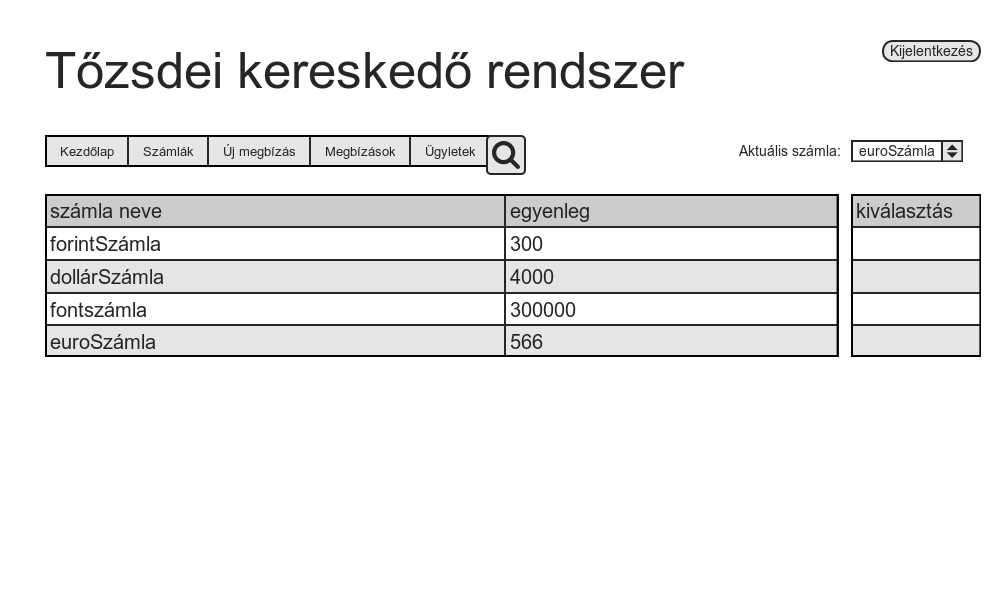
\includegraphics[width=150mm, keepaspectratio]{figures/user_1/bills.png}
\caption{Ügyfél számlái}
\label{fig:haromreteg}
\end{figure}

\subsection{Ügyfél megbízásai}
A bróker is egy hasonló oldalt lát az ügyfelek megbízásairól.

\begin{figure}[!ht]
\centering
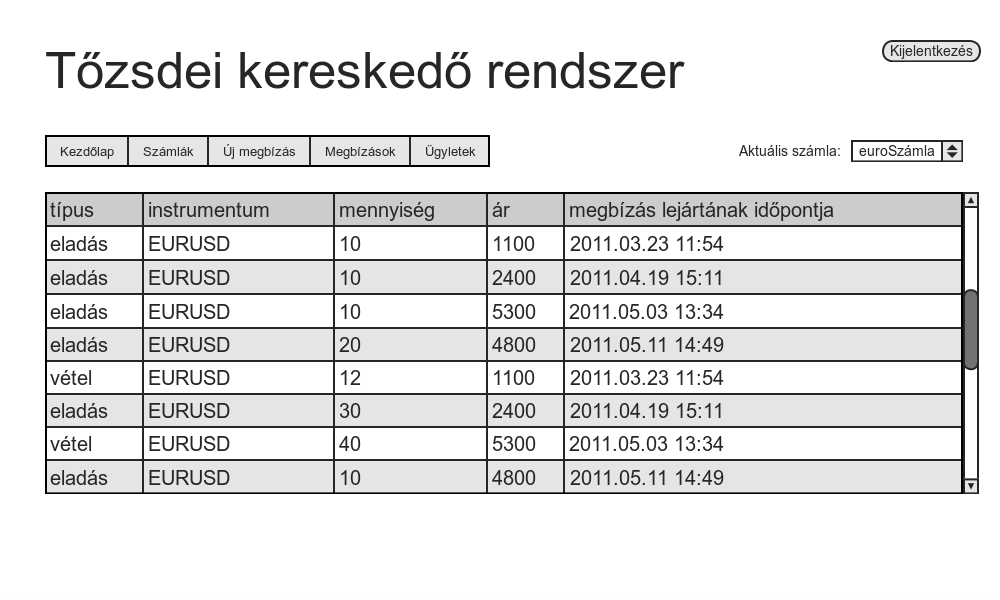
\includegraphics[width=150mm, keepaspectratio]{figures/user_1/megbizasok.png}
\caption{Ügyfél megbízásai}
\label{fig:haromreteg}
\end{figure}


\subsection{Ügyfél ügyletei}
A bróker is egy hasonló oldalt lát az ügyfelek ügyleteiről.

\begin{figure}[!ht]
\centering
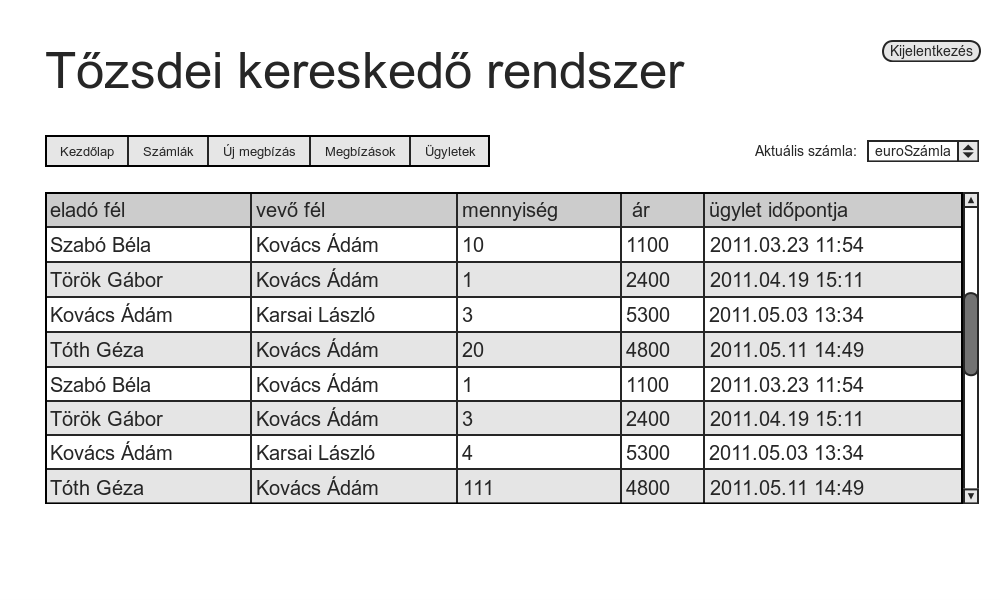
\includegraphics[width=150mm, keepaspectratio]{figures/user_1/ugyletek.png}
\caption{Ügyfél ügyletei}
\label{fig:haromreteg}
\end{figure}

\subsection{Új megbízás}

\begin{figure}[!ht]
\centering
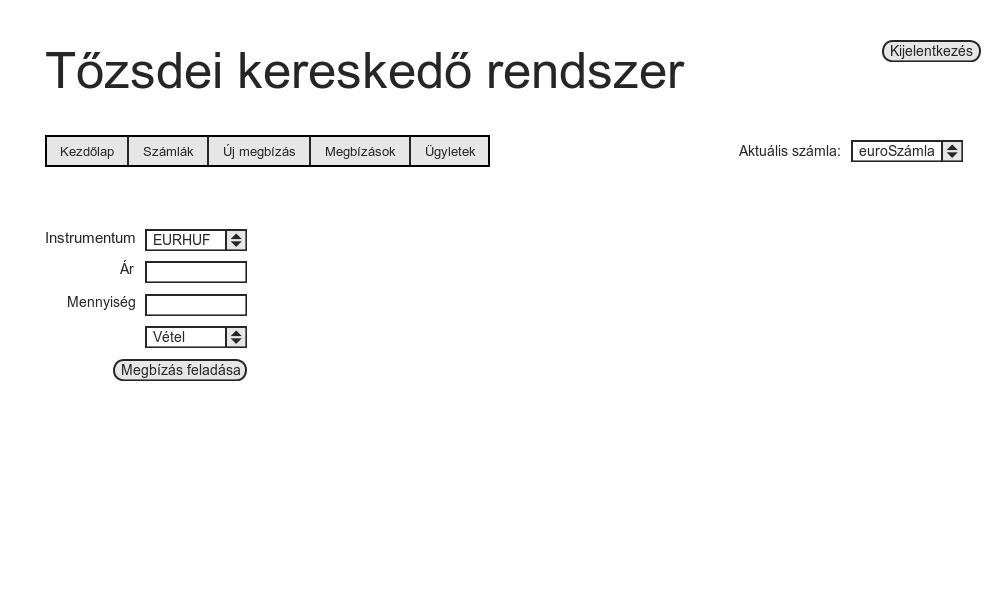
\includegraphics[width=150mm, keepaspectratio]{figures/user_1/uj_megbizas.png}
\caption{Új megbízás}
\label{fig:haromreteg}
\end{figure}

%,,,,,,,,,,,,,,,,,,,,,,,,,,,,,,,,,,,,,,,,,,,,,,,,,,,,,,,,,,,,,,,,,,,,,,,,,,,,
\section{Biztonsági követelmények}\label{sect:security}
%,,,,,,,,,,,,,,,,,,,,,,,,,,,,,,,,,,,,,,,,,,,,,,,,,,,,,,,,,,,,,,,,,,,,,,,,,,,,

\subsection{Authentikáció}
Biztonsági szempontból a legfontosabb, hogy illetéktelen személyek ne tudjanak belépni mások felhasználói fiókjába, így számukra kedvezőtlen megbízásokat indítani vagy a számlájukról pénzt lopni. Természetesen az adminisztrátori szerepkörben lévő felhasználó védelme a legfontosabb, így ott érdemes akár valamilyen fizikai (token kulcs) authentikáció használata. Mivel a rendszer nagyon sok pénzt kezelhet, így ilyen fizikai kulcsot akár minden felhasználó kaphatna a végleges rendszerben.

\subsection{Authorizáció}
A felhasználói szerepeknek élesen, pontosan el kell különülniük és implementálás után az egyes jogokat megfelelően ki kell tesztelni, így megakadályozható, hogy egy felhasználó egy másik felhasználó számlájához hozzáférhessen, esetleg megbízásokat indítson onnan vagy egyszerűen csak olyan adatokhoz jusson hozzá ami nem az ő tulajdona.

\subsection{Beviteli mezők védelme}
Természetesen a különböző beviteli mezőket védeni kell, mind SQL Injection , mind XSS ellen, így megakadályozva, hogy illetéktelen kód fusson az adatbázison vagy a kliens böngészőjében.  A kirívóan magas (a felhasználó számlájához képest) összegű megbízásokra érdemes külön visszaigazolást kérni, így elkerülhetők figyelmetlenségből, elgépelésből adódó nagyobb veszteségek.

\subsection{Biztonságos kommunikáció}
Annak érdekében, hogy egy harmadik fél ne halgathassa le a szerver-böngésző kommunikációt érdemes titkosított kapcsolatot alkalmazni, így megakadályohatjuk mind, hogy harmadik félhez illetéktelen adatok kerüljenek ki, mind, hogy egy harmadik fél a kommunikáció közepébe álljon és hamis információkat adjon a felhasználónak vagy a szervernek (pl: magasabb összzegű megbízás a felhasználó tudta nélkül).
A rendszernek rendelkeznie kell egy hivatalos harmadik fél által kiadott tanusítvánnyal ami biztosítja a felhasználót, hogy a biztonságos hálózati kommunikáció során nem egy hamis renszerrel kommunikál, hanem a valódival.

%,,,,,,,,,,,,,,,,,,,,,,,,,,,,,,,,,,,,,,,,,,,,,,,,,,,,,,,,,,,,,,,,,,,,,,,,,,,,
\section{Tervezett architektúra}\label{sect:designed_architecture}
%,,,,,,,,,,,,,,,,,,,,,,,,,,,,,,,,,,,,,,,,,,,,,,,,,,,,,,,,,,,,,,,,,,,,,,,,,,,,

A rendszert egy három rétegű architektúrában valósítjuk meg. A megjelenítést a felhasználó böngészőjében (kliens oldaon) végezzük, az üzleti logikát (megbízások, ügyletek kezelése) egy dedikált szerveren, míg az adatokat egy adatbázis rétegben tároljuk.
Az alkalmazás egy webalkalmazás lesz, a Ruby on Rails keretrendszer lesz az alapja, így a működése platformtól független lesz. 

Az alkalmazás frontendje és üzleti logikája mögött egy SQL (MySQL vagy PostgreSQL) adatbázis fog futni.

Az adatbázisban tároljuk a felhasználók rekordjait, az ügyfelek számláit és az ezekhez tartozó megbízások és ügyletek rekordjait. Új felhasználó regisztrációjakor, új számla létrehozásakor, egy megbízás feladásakor vagy egy ügylet megkötésekor egy új bejegyzés jön létre az adatbázisban, ezeket különböző felületeken a felhasználók listázzák, egyes mezőket szerkeszthetnek, felülírhatnak vagy akár törölhetnek is. A különböző entitások között tartalmazó kapcsolatok lehetnek, melyeket figyelembe kell venni az adatbázis tervezésekor.

Az adatbázisból kiolvasott és éppen használatban lévő adatokat a memóriában tároljuk, mint amilyen az aktuálisan belépett felhasználó adatai vagy az aktuálisan kiválasztott számlához tartozó információ. Ezekkel az adatokkal folyamatosan dolgozunk, így megéri őket a memóriában tartani, adatbázis hívást csak entitások listázása, új entitás létrehozása, módosítása vagy törlése esetén hívunk, módosító műveleteknél a memóriában és az adatbázisban tárolt adatok szinkronitásáról gondoskodunk.

A részvények aktuális árfolyamát a Google Finance API fogja nyújtani JSON formátumban, ezt az adatot nem szükséges az adatbázisba kimenteni, hiszen folyamatosan változik, a web service által visszaadott értékek érvényességi idejük alatt a memóriában lesznek tárolva, innen kérdezheti őket a webalkalmazás. A memóriában tárolt értékek periodikusan frissítve lesznek.


\begin{figure}[!ht]
\centering
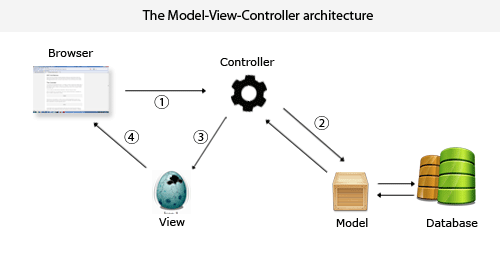
\includegraphics[width=150mm, keepaspectratio]{figures/arch.png}
\caption{Architektúra}
\label{fig:haromreteg}
\end{figure}
%%----------------------------------------------------------------------------
\chapter{Rendszerterv}\label{sect:rszterv}
%----------------------------------------------------------------------------

Jelen fejezetben szeretnénk bemutatni az elkészítendő rendszer tervét. A következő részek kitérnek az architektúra kiválasztására és megvalósítására (\sectref{architektura} szakasz), az itt szereplő rétegek felépítésére és funkciójára (\sectref{retegek} szakasz), valamint végül a program funkcióinak ismertetésére (\sectref{rsz_funkciok} szakasz).

%,,,,,,,,,,,,,,,,,,,,,,,,,,,,,,,,,,,,,,,,,,,,,,,,,,,,,,,,,,,,,,,,,,,,,,,,,,,,
\section{Architektúra}\label{sect:architektura}
%,,,,,,,,,,,,,,,,,,,,,,,,,,,,,,,,,,,,,,,,,,,,,,,,,,,,,,,,,,,,,,,,,,,,,,,,,,,,


Az alkalmazás három rétegből épül fel a klasszikus MVC architektúra alapján. A kliens oldalon a felhasználó webböngészőben futtatja az alkalmazást. A szerver oldali kód egy Apache Web Serveren fog futni, mely többszálú kliens kiszolgálást tesz lehetővé és képes titkosított csatornán végezni a kommunikációt a köztes rétegben, nagyban növelve a privát adatok védelmét. Az modell réteg a PostgreSQL adatbázis kezelő rendszeren alapul, mely egy széles körben támogatott open-source megoldás, mely megfelelő hatékonységgal képes szolgálni a rendszert. 

%. . . . . . . . . . . . . . . . . . . . . . . . . . . . . . . . . . . . . .
%\subsubsection{Egy subsubsection}\label{sect:egysubsubsection}
%. . . . . . . . . . . . . . . . . . . . . . . . . . . . . . . . . . . . . .

%,,,,,,,,,,,,,,,,,,,,,,,,,,,,,,,,,,,,,,,,,,,,,,,,,,,,,,,,,,,,,,,,,,,,,,,,,,,,
\section{Rétegek}\label{sect:retegek}
%,,,,,,,,,,,,,,,,,,,,,,,,,,,,,,,,,,,,,,,,,,,,,,,,,,,,,,,,,,,,,,,,,,,,,,,,,,,,

 A megjelenítési réteg a kliens oldalon játszik fő szerepet, ahol a rendszer felhasználója egy tetszőleges böngészőben futtathatja a webalkalmazást. Az üzleti logikai funckiók a szerver oldalon futnak, a webalkalmazáshoz egy dedikált szerver tartozik, mely képes több kliens egyidejű kiszolgálására. Ide érkeznek be kliens oldalról a kérések, az üzleti logikai rétegen keresztül tudunk szolgáltatásokat nyújtani a kliens felé. A felhasználók perzisztens adataira, a különböző megbízások és ügyletek adatainak tárolására egy adatbázis és a programozható kezelőfelülete áll rendelekezésünkre.

%............................................................................
\subsection{Megjelenítési réteg}\label{sect:kliens_reteg}
%............................................................................

Az felhasználó számítógépén, egy tetszőleges böngészőben fut az alkalmazás kliens rétege, ami a vizuális megjelenítésért felelős és kapcsolódásokat definiál az üzleti logika réteg felé.

Az alkalmazás a legmodernebb webes trendeket követi, szem előtt tartva a minél nagyobb körű kompatibiltást különböző böngészőkkel. A felhasználóhoz érkező végső termék egy HTML lap CSS stíluslapokkal és Javascript kódokkal megtámogatva. 
A CSS fájlok felelnek a felhaszálói felületen elhelyezett elemek beállításáért, segítséget nyújtanak egy koherens design megalkotásában, ahol az elemek vizuális tulajdonságai teljes mértékben lecsatolódnak az elemek definiálásától.
A HTML kódban hozunk létre elemeket a kliens alkalmazás felhasználói felületén. Az elemek lehetnek statikus vagy interaktív elemek, utóbbiakkat használva a felhasználó az üzleti logika felé kérésekkel fordulhat, melyekre a szerver válaszol egy újabb HTML fájllal. A felhasználó nem csak újabb oldalakra léphet tovább, hanem adatokat is küldhet, az üzleti logika által nyújtott felületen keresztül manipulálhatja a modell rétegben található adatokat, ha rendelkezik az ehhez megfelelő jogosultságokkal.

\bigskip

A webalkalmazás a kliens-szerver alapokon nyugvó REST architektúrán alapul, amelynek legfontosabb tulajdonsága, hogy minden fogalmát és objektumát a rendszernek erőforrással reprezentáljuk, melyeken különböző műveleteket végezhetünk, ezzel manipulálva a reprezentációt. A kliens oldalon a webböngésző különböző HTTP metódusokat (GET, POST, PUT, DELETE) küldve végezheti ezeket a műveleteket, melyeket az üzleti logika rész megfelelő funkciókhoz irányít.

%............................................................................
\subsection{Webszerver réteg}\label{sect:szerver_reteg}
%............................................................................

A kontroller réteget egy webszerver valósítja meg, melynek feladata a klienstől beérkező kérések és adatok feldolgozása, adatbázis manipulációk kezdeményezése és a válaszok visszaküldése a kliens réteg felé.

A webszerver legkülső felülete egy routing tábla, mely a klienstől érkező, egyes erőforrásokon végzett kéréseket a megfelelő funkcióhoz rendeli. Ezek a funkciók szintén az üzleti logika rétegben vannak definiálva, a különböző erőforrás reprezentációkhoz megfelelő modellek vannak definiálva. A modelleken az objektum-orientált szemléletet követve attribútumok és funckiók vannak definálva. Az osztályok és attribútumok közvetlen kapcsolatban állnak az adatbázis egyes tábláival, definiálhatunk ezen túl egy-egy, egy-több és több-több kapcsolatokat, melyek az adatbázis rétegben kapcsolótáblák segítségével jelennek meg, de az üzleti logika réteg számára ez a működés transzparens.

%............................................................................
\subsection{Adatbázis réteg}\label{sect:adatbazis_reteg}
%............................................................................

Az adatbázisban az üzleti logika részben definiált osztályok tábla reprezentációi szerepelnek, a köztük levő kapcsolatokat megvalósító kapcsolótáblák és különböző segédtáblák, melyek csupán a működést támogatják. Az adatbázisban egy tábla egy erőforrás osztálynak felel meg, ezen osztályok példányai a megfelelő tábla egy sorában vannak tárolva, az osztályok attribútumainak a tábla oszlopai felelnek meg.

A USER tábla tartalmazza a regisztrált felhasználókat, a jelszavakat lekódolva tároljuk az esetleges sikeres támadás hatásainak tompítása érdekében. A bejelentkezéshez kapcsolatos adatok és a felhasználó egyéb adatai tárolódnak ebben a táblában, továbbá egy flag, mely jelzi, hogy a felhasználó regisztrációját aktiválva van-e.

A ROLE tábla tartalmazza a rendszerben megtalálható szerepeket, az adminisztátor, bróker és felhasználó szerep elérhető jelenleg a rendszerben. A felhasználók és szerepek között több-több kapcsolat van, ezt a USER\_ROLE kapcsolótábla valósítja meg. 

Minden felhasználóhoz tartozhat több számla, így az ACCOUNT tábla a számla adatai mellett egy referenciát is tartalmaz a megfelelő felhasználóra.

A STOCK tábla különböző részvényeket reprezentál, mely alapvető adatokat tartalmaz a részvényről (név, aktuális árfolyam, különböző időbélyegek).

A STOCK\_VOL tábla az egyes számlákhoz tartozó részvények számát tárolja, így tárolja a számla és a részvény azonosítóját, illetve egy mennyiséget, ami a részvények számát jelzi.

A TRANSACTIONS tábla tartalmazza a már megkötött ügyleteket egy referenciával a megfelelő részvény típusra. Ezen kívül különböző időbélyegeket és az ügylet árát tartalmazza.

Az ORDERS tábla a megrendeléseket tartalmazza, egy megrendelés egy számlához tartozik, így a megfelelő oszlopban hivatkozik egy számlára. Ezen kívül egy ügylet referenciát is tartalmaz, mely NULL értéket tartalmaz, ha az ügylet még nem jött létre. A harmadik referencia a megrendelt részvényre mutat, ezentúl tartalmazza a megrendeléshez tartozó egyéb információkat (ár, vétel-eladás flag, időbélyegek).

%,,,,,,,,,,,,,,,,,,,,,,,,,,,,,,,,,,,,,,,,,,,,,,,,,,,,,,,,,,,,,,,,,,,,,,,,,,,,
\section{Biztonság és skálázhatóság}\label{sect:rsz_funkciok}
%,,,,,,,,,,,,,,,,,,,,,,,,,,,,,,,,,,,,,,,,,,,,,,,,,,,,,,,,,,,,,,,,,,,,,,,,,,,,
A rendszert a Heroku web kiszolgáló felhőjébe telepítettük, így egyszerre kaptunk nagy skálázhatóságot (tetszőleges méretű adatbázis, tetszőleges mennyisgű adatbázis szál, illetve HTTP kérés kiszolgáló), illetve biztonságot (HTTPS-en keresztüli elérés).

A rendszerben lévő modellekhez kizárólag authentikáció után lehet hozzáférni, illetve deklaratívan le van fektetve melyik felhasználói szerepkör melyik modellhez, milyen formán (létrehozás, módosítás, listázás, törlés) férhet hozzá. Az SQL injection támadások ellen a Rails beviteli mezői automatikusan védenek.

%,,,,,,,,,,,,,,,,,,,,,,,,,,,,,,,,,,,,,,,,,,,,,,,,,,,,,,,,,,,,,,,,,,,,,,,,,,,,
\section{Funkciók}\label{sect:rsz_funkciok}
%,,,,,,,,,,,,,,,,,,,,,,,,,,,,,,,,,,,,,,,,,,,,,,,,,,,,,,,,,,,,,,,,,,,,,,,,,,,,

\subsection{Regisztráció kérelme}
A felhasználó egy felületen a szükséges adatok bevitelével regisztrációt kérvényez (név, email cím, jelszó). A felhasználó ekkor még inaktív állapotban lesz, az adminisztrátornak kell aktiválnia, illetve a megfelelő szerepkört hozzárendelnie.
\newline \underline{Szerepkör}: Ügyfél, Adminisztrátor, Bróker

\subsection{Felhasználó regisztrációja}
A felhasználó a beérkezett regisztrációs kérelmet feldolgozza és létrehoz egy új felhasználót, a role alapvetően ügyfél típusú lesz, de az adminisztrátor átállíthatja. Regisztráció után a felhasználó inaktív állapotban lesz, az adminisztrátornak aktiválnia kell belépéshez.
\newline \underline{Szerepkör}: Adminisztrátor

\subsection{Ügyfél számla kezelése}
Az ügyfél létrehozhat magának tetszőleges mennyiségű számlát amire pénzt tölthet, majd ezt szerkesztheti (pénzt tölt fel, vesz le), törölheti, listázhatja. A számlát aktiválhatja ekkor az lesz az alapértelmezett számla minden művelethez.
\newline \underline{Szerepkör}: Ügyfél

\subsection{Megbízás kezelése}
 A felhasználó kitölt egy megbízási formulát, melyhez megadja a szükséges adatokat(számla, részvény, ár, megbízás tipusa: vétel/eladás), majd ezt beregisztrálja a rendszerbe. A megbízást addig módosíthatja a felhasználó amíg nem lesz belőle ügylet, addig akár törölheti is. Vételi megbízáskor a szükséges mennyiségű pénz azonnal eltávolítódik a számlárol, csak akkor kerül vissza, ha a megbízás törlődik. Eladási megbízásnál az ügylet létrejöttekor kerül a pénz a számlára (ahonnan a részvény véve lett). Megbízást indíthatunk a főoldalról is az 'Eladás' vagy 'Vétel' gomb megnyomásával, ekkor az aktuális árfolyamon az aktivált számláról indul a megbízás.
\newline \underline{Szerepkör}: Ügyfél

\subsection{Részvények árfolyamának megtekintése}
A fő oldalon a felhasználók láthatják a tőzsdén lévő összes részvény múltbéli árát egy grafikon segítségével. A bal oldali listából választhatják ki, hogy éppen melyik részvényt mutassa a grafikon.
\newline \underline{Szerepkör}: Ügyfél

\subsection{Ügyfelek kezelése}
A brókerek látják az összes felhasználót, listázhatják számláikat, megbízásaikat, ügyleteiket. Megbízásaikat akár módosíthatják is.
\newline \underline{Szerepkör}: Bróker

%%----------------------------------------------------------------------------
\chapter{Telepítési dokumentáció}\label{sect:telepites}
%----------------------------------------------------------------------------

Az alkalmazást természetéből adódóan egy webszerverre szükséges telepíteni, ez célszerűen a Microsoft IIS 7-es verziója. A telepítéshez a webprojekt könyvtárának tartalmát kell elérhetővé tenni a webszerveren. Célszerű a könyvtárban található HTML, vagy ASPX fájlt a könyvtár default kezdőlapjának beállítani, így a \texttt{kiszolgáló/elérésiút} címen az alkalmazás könnyen indítható.

A program működése emellett természetesen igényli a felhasználó számítógépén a Silverlight környezet meglétét. Azonban ha nem érzékeli, a kezdőlapon automatikusan felajánlja a letöltést és telepítést, ami után a rendszer rögtön használhatóvá válik.

%----------------------------------------------------------------------------
\chapter*{Értékelés}\label{sect:ertekeles}
%----------------------------------------------------------------------------

A házi feladat elkészítése során végigvittük egy alkalmazás megvalósítását az abasztrakt leírástól a működő alkalmazásig és az őt leíró dokumentáció elkészítéséig. A kezdeti személyes kontaktus és az előzetes megbeszélések után kihasználtuk a GIT verziókezelő és hálózati kommunikációs technológiák előnyeit, így távolról tudtunk dolgozni a közös projekten, miközben folyamatos virtuális kapcsolatban voltunk egymással. A munka során a követelményspecifikációban lefektetett terveket és elképzeléseket sikerült megvalósítani, megismerkedtünk néhány új fogalommal, az eddigi tudásunkat pedig tovább mélyítettük a már ismert technológiákkal kapcsolatban is. Remélhetőleg az itt szerzett tapasztalatokat későbbi munkáink során hatékonyan kamatoztathatjuk, amennyiben a mostanihoz hasonló komplex tervezést, együttműködést és kiviteleyést igénylő feladatokkal találjuk magunkat szembe.

%,,,,,,,,,,,,,,,,,,,,,,,,,,,,,,,,,,,,,,,,,,,,,,,,,,,,,,,,,,,,,,,,,,,,,,,,,,,,
\subsubsection{Továbbfejlesztési lehetőségek}\label{sect:tovabbfejlesztes}
%,,,,,,,,,,,,,,,,,,,,,,,,,,,,,,,,,,,,,,,,,,,,,,,,,,,,,,,,,,,,,,,,,,,,,,,,,,,,

A szoftver jelenleg az aktuális árfolyamok számítására egy egyszerű modellt használ, mely a valóságban jóval bonyolultabban működik. A valós adatok részletes tanulmányozásával valószínüleg jóval komplexebb és reálisabb leíró modellt tudnánk alkotni, amely meghatározza a tőzsdei árfolyamok változásának mechanizmusait. 
Jeleneg egy egyszerű, de átlátható kezelőfelülettel rendelkezik az alkalmazás. Egy hivatalos designer egyedi és divatos megjelenést szabhatna az oldalnak, mellyel fokozhatná mind a használhatóságot, mind a kényelmet, mind az esztétikai élvezetet az oldal használata közben.
A megoldás nincsen felkészülve nagy tömegek kiszolgálására, nincs optimalizálva a válaszidők minimalizálására és kiélezve a hatékonyságra. Minden olyan egyszerűen és egyértelműen van megoldva, hogy átlátható és redundanciától lehetőleg mentes legyen, de egy teljesítmánykritikus rendszer esetében sok optimalizációs lehetőség rendelkezésünkre áll. 


%\phantomsection\markboth{Ábrák jegyzéke}{}\listoffigures\newpage
%\phantomsection\markboth{Táblázatok jegyzéke}{}\listoftables\newpage

%\phantomsection\markboth{Irodalomjegyzék}{}\bibliography{mybib}
%%\addcontentsline{toc}{chapter}{Irodalomjegyzék}
%\bibliographystyle{unsrt}

\label{page:last}
\end{document}
